% IEEE formatında Türkçe kısa rapor (ham taslak)
\documentclass[10pt,twocolumn]{article}
\usepackage[T1]{fontenc}
\usepackage[utf8]{inputenc}
\usepackage{lmodern}
\usepackage{geometry}
\geometry{a4paper,margin=0.75in}
\usepackage{graphicx}
\usepackage{amsmath}
\usepackage{booktabs}
\usepackage[hidelinks]{hyperref}
\usepackage{caption}

\title{Lojistik Regresyon ile İşe Alım Tahmini: Eğitim, Doğrulama ve Test Değerlendirmesi}
\author{Muhammed Kayra Bulut -- 25501805}
\date{}

\begin{document}
\maketitle

\begin{abstract}
\noindent Bu çalışmada iki sınav puanından yola çıkarak işe alım (0/1) kararını tahmin eden lojistik regresyon modeli eğitilmiş ve değerlendirilmiştir. Veri kümesi 100 örnekten oluşmakta; bunların 60'ı işe alınmış, 40'ı ise alınmamıştır. Eğitim sürecinde kayıp ve başarım eğrileri izlenmiş, modelin aşırı uyum sergilemediği gözlemlenmiştir. Deneysel sonuçlar; eğitim, doğrulama ve test bölümlerine ait doğruluk, kesinlik, duyarlılık ve F1 skorlarını kapsamaktadır. Doğrulama başarımının 0.95 civarında plato yapması ve 500. döngüden sonra marjinal kazanımların azalması, daha uzun eğitimlerin pratik faydasının sınırlı olduğunu göstermektedir.
\end{abstract}

\textbf{Anahtar Sözcükler---}lojistik regresyon, sınıflandırma, doğruluk, kesinlik, duyarlılık, F1 skoru, aşırı uyum

\section{Giriş}
Bu ödevde amaç; iki boyutlu özelliklerden (\texttt{exam\_1}, \texttt{exam\_2}) işe alım kararını tahmin etmektir. Problem ikili sınıflandırmadır ve model olarak gradyan iniş ile eğitilen lojistik regresyon kullanılmıştır. Lojistik regresyon, sigmoid fonksiyonu ($\sigma(z) = \frac{1}{1 + e^{-z}}$) aracılığıyla lineer kombinasyonu 0 ile 1 arasında bir olasılık değerine dönüştürerek sınıflandırma yapan yaygın bir istatistiksel öğrenme yöntemidir.

Veri kümesi toplam 100 gözlem içermektedir; genel dağılım \textbf{60 işe alınan} (pozitif sınıf, $y=1$) ve \textbf{40 alınmayan} (negatif sınıf, $y=0$) şeklindedir. Veriler; tabakalı (stratified) şekilde yüzde 60 eğitim (60 örnek), yüzde 20 doğrulama (20 örnek), yüzde 20 test (20 örnek) olarak bölünmüştür. Bu bölünme sınıf oranlarını koruyacak şekilde yapılmıştır; her bir bölümde örneklerin yüzde 60'ı işe alınmış, yüzde 40'ı ise alınmamış statüsündedir.

\section{Deneysel Analiz}
\subsection{Veri Bölümlerinin Homojenliği}
Eğitim, doğrulama ve test setlerinin saçılım grafikleri \emph{Şekil~\ref{fig:train-scatter}}, \emph{Şekil~\ref{fig:val-scatter}} ve \emph{Şekil~\ref{fig:test-scatter}}'da ayrı ayrı gösterilmiştir. Üç bölüm de genel dağılım açısından homojendir; her birinde işe alınan ve alınmayan örneklerin sınav puanı aralıkları örtüşmekle birlikte, işe alınanlar üst bölgede kümelenmektedir. Bu yatay homojenlik, tabakalı bölmenin sınıf oranlarını koruduğunu doğrulamaktadır.

Görsel inceleme, verilerin lineer olarak tam ayrılabilir olmadığını ancak \textbf{neredeyse lineer ayrılabilir} (nearly linearly separable) bir yapı sergilediğini göstermektedir. İki sınıf arasındaki karar sınırı (decision boundary), bir doğru ile makul bir şekilde çizilebilir düzeydedir. Bu durum, lojistik regresyon gibi lineer sınıflandırıcıların bu veri seti üzerinde başarılı olmasını mümkün kılmaktadır. Ayrıca, her üç bölümde de benzer geometrik yapının korunmuş olması, modelin eğitim sürecinde öğrendiği desenin diğer bölümlerde de geçerli olacağını göstermektedir.

\subsection{Eğitim Dinamikleri: Kayıp ve Başarım}
Kayıp ve başarım eğrileri \emph{Şekil~\ref{fig:loss}} ile \emph{Şekil~\ref{fig:accuracy}}'da ayrı ayrı sunulmuştur. Model, ikili çapraz-entropi (binary cross-entropy) kayıp fonksiyonu ile optimize edilmiştir. Eğitim kaybı başlangıçta hızlı düşmekte, doğrulama kaybı ise daha düşük seviyelere oturarak \emph{erken ve kararlı} bir yakınsama göstermektedir. Bu durum, doğrulama setinin eğitim setine kıyasla daha "kolay" bir yapıya sahip olabileceğini veya modelin bu örnekler üzerinde daha güvenli tahminler ürettiğini düşündürmektedir.

Başarım tarafında eğitim eğrisi 0.88--0.90 bandında plato yaparken, doğrulama başarımı 0.95 civarında sabitlenmektedir. Bu iki eğri arasındaki farkın küçük kalması ve doğrulama başarımının düşmemesi, \textbf{aşırı uyum (overfitting) gözlemlenmediğini} işaret etmektedir. Aşırı uyumun görülmemesi, modelin kapasitesinin veri kümesinin karmaşıklığı ile iyi dengelendiğini göstermektedir. Lojistik regresyon gibi basit parametrik modellerin, küçük ve orta ölçekli veri setlerinde aşırı uyum riskini doğal olarak sınırladığı bilinmektedir.

Ayrıca eğriler 500. döngü civarında belirgin biçimde satürasyona ulaşmakta, bu noktadan sonra iyileşme marjinal kalmaktadır. Bu gözlem, erken durdurma (early stopping) stratejilerinin kullanılabileceğini ve eğitim süresinin 500--700 döngü ile sınırlandırılmasının yeterli olacağını göstermektedir. Daha uzun eğitimlerin hesaplama maliyeti artırmasına rağmen, model performansına anlamlı katkı sağlamadığı görülmektedir.

\begin{figure}[!htb]
  \centering
  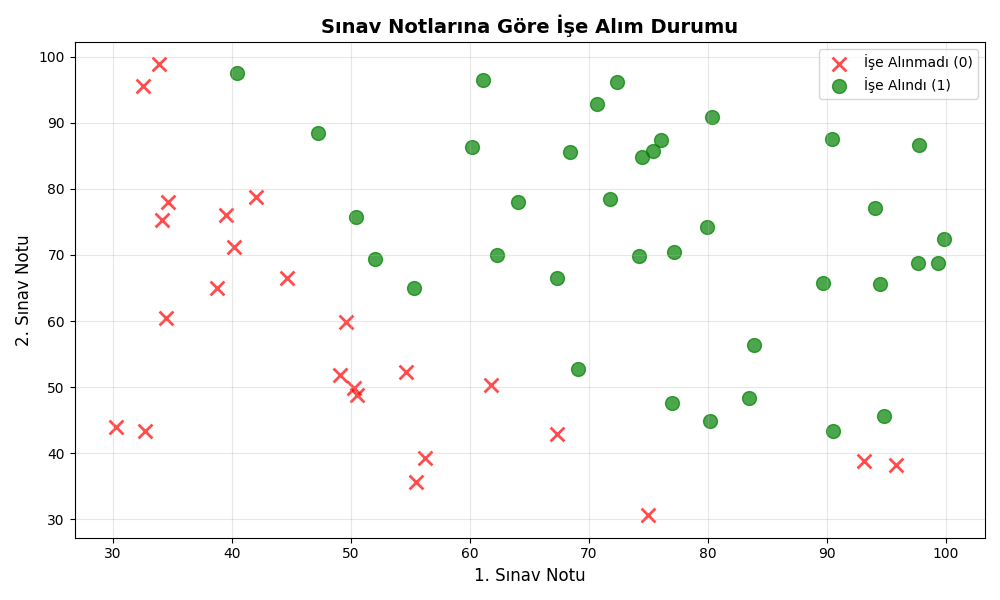
\includegraphics[width=0.9\linewidth]{dataset/gorseller/train_data_plot.png}
  \caption{Eğitim veri seti saçılım grafiği. Sınıflar birbirine yakın fakat ayrılabilir bölgeler oluşturuyor.}
  \label{fig:train-scatter}
\end{figure}

\begin{figure}[!htb]
  \centering
  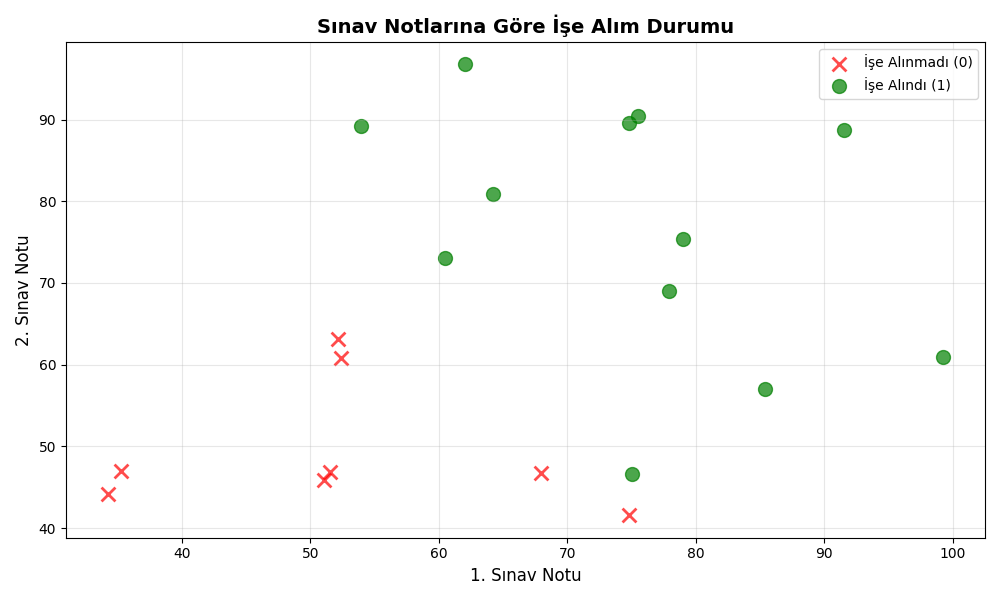
\includegraphics[width=0.9\linewidth]{dataset/gorseller/validation_data_plot.png}
  \caption{Doğrulama veri seti saçılım grafiği. Eğitim setindeki desenin homojen biçimde korunduğu görülüyor.}
  \label{fig:val-scatter}
\end{figure}

\begin{figure}[!htb]
  \centering
  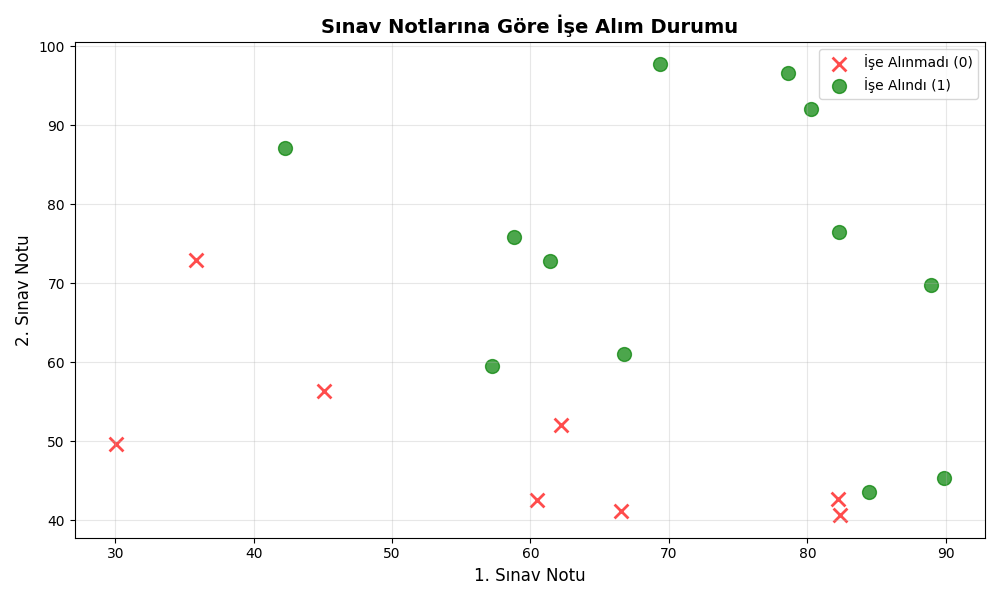
\includegraphics[width=0.9\linewidth]{dataset/gorseller/test_data_plot.png}
  \caption{Test veri seti saçılım grafiği. Homojen dağılım, genelleme değerlendirmesini güvenilir kılıyor.}
  \label{fig:test-scatter}
\end{figure}

\begin{figure}[!htb]
  \centering
  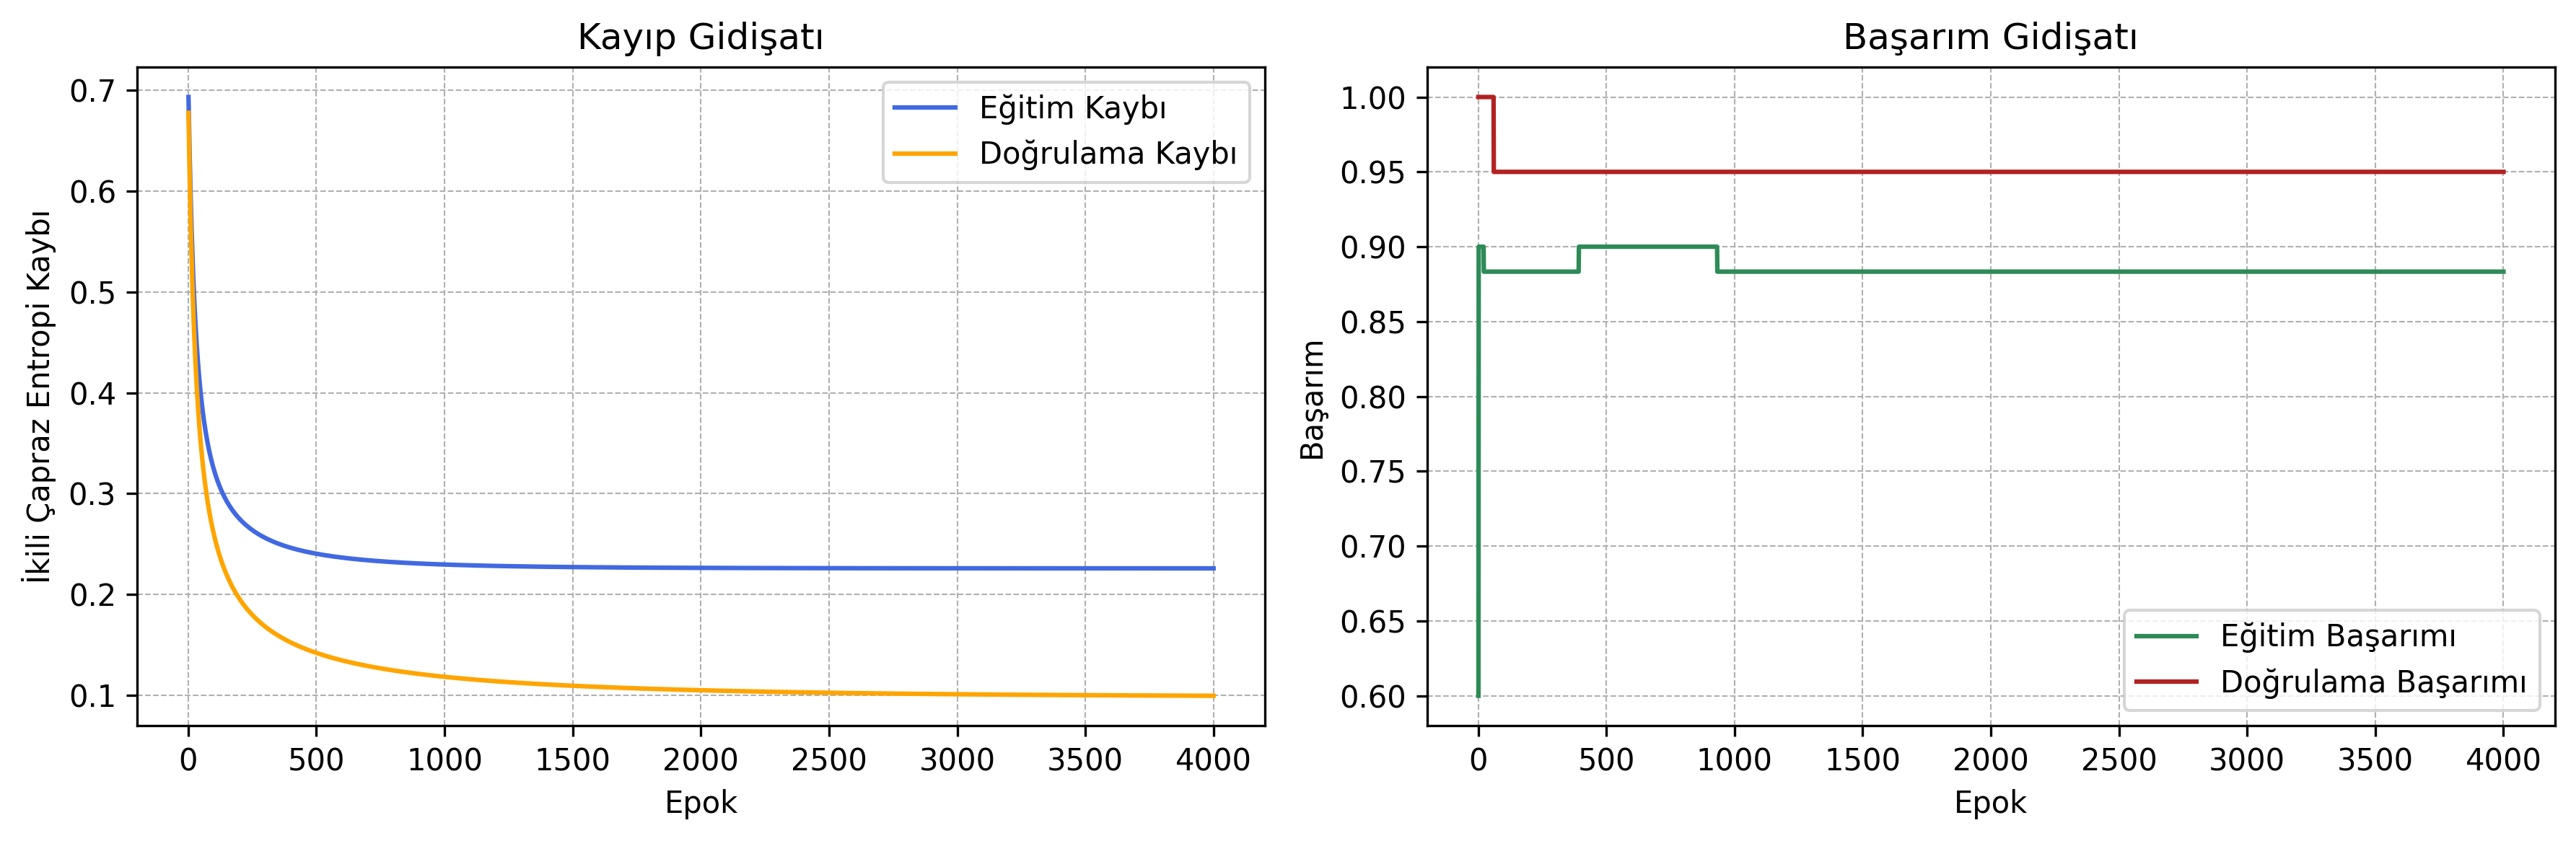
\includegraphics[width=0.9\linewidth]{dataset/gorseller/egitim_dogrulama_olcutler.png}
  \caption{Eğitim ve doğrulama kayıplarının evrimi. Doğrulama kaybı erken aşamada kararlı seviyeye inmektedir.}
  \label{fig:loss}
\end{figure}

\begin{figure}[!htb]
  \centering
  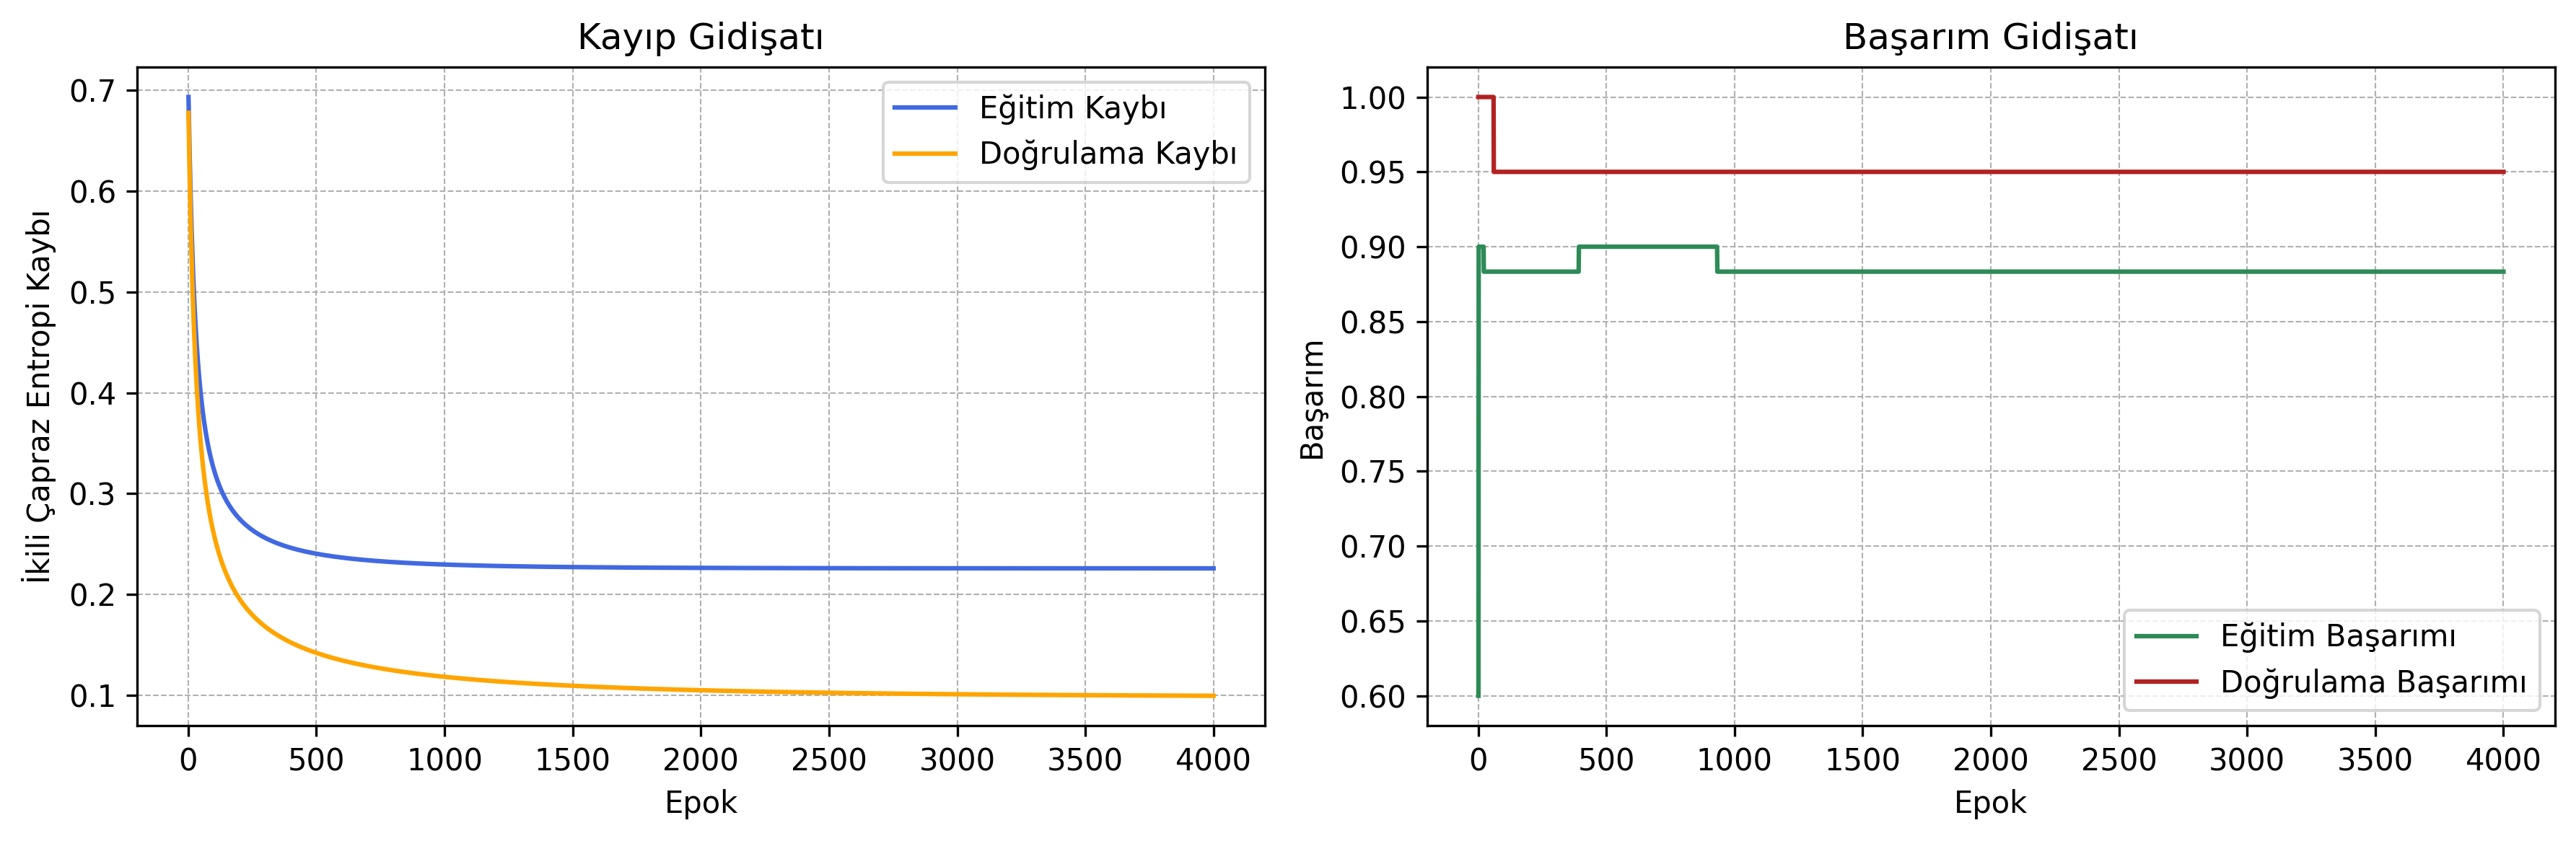
\includegraphics[width=0.9\linewidth]{dataset/gorseller/egitim_dogrulama_olcutler.png}
  \caption{Eğitim ve doğrulama başarımının (accuracy) evrimi. Doğrulama başarımı 0.95 civarında plato yapmaktadır.}
  \label{fig:accuracy}
\end{figure}

\subsection{Nihai Ölçütler: Accuracy, Precision, Recall, F1}
Her bir bölüm (eğitim/doğrulama/test) için hesaplanan ölçütler \emph{Tablo~\ref{tab:metrics}}'te özetlenmiştir. Bu ölçütler, modelin farklı açılardan değerlendirilmesini sağlamaktadır:

\begin{itemize}
\item \textbf{Doğruluk (Accuracy):} Tüm tahminler içinde doğru sınıflandırılan örneklerin oranı. Genel başarımın en basit göstergesidir.
\item \textbf{Kesinlik (Precision):} Pozitif olarak tahmin edilen örnekler içinde gerçekten pozitif olanların oranı. Yanlış pozitif (false positive) oranını düşük tutmanın önemli olduğu durumlarda kritiktir.
\item \textbf{Duyarlılık (Recall):} Gerçekte pozitif olan örnekler içinde doğru şekilde pozitif olarak tahmin edilenlerin oranı. Yanlış negatif (false negative) oranını minimize etmek önemliyse bu ölçüt ön plana çıkar.
\item \textbf{F1 Skoru:} Kesinlik ve duyarlılığın harmonik ortalaması. Dengesiz veri setlerinde veya hem kesinlik hem duyarlılığın önemli olduğu durumlarda tercih edilir.
\end{itemize} 

\begin{table}[!htb]
  \centering
  \caption{Bölümlere göre ölçütler.}
  \label{tab:metrics}
  \begin{tabular}{lcccc}
  \toprule
  Bölüm & Doğruluk & Kesinlik & Duyarlılık & F1 \\
  \midrule
  Eğitim & 0.8833 & 0.8919 & 0.9167 & 0.9041 \\
  Doğrulama & 0.9500 & 1.0000 & 0.9167 & 0.9565 \\
  Test & 0.8500 & 0.8462 & 0.9167 & 0.8800 \\
  \bottomrule
  \end{tabular}
\end{table}

\emph{Şekil~\ref{fig:train-bars}}'da gösterilen eğitim bölümü ölçütlerine bakıldığında; doğruluk, kesinlik, duyarlılık ve F1 skorları 0.88--0.92 bandında toplanmaktadır. Ancak eğitim seti modelin eğitimi esnasında gördüğü örneklerden oluştuğundan, bu ölçütlerin değerlendirilmesinde dikkatli olunmalıdır. Eğitim başarımı, modelin veriyi ne kadar iyi ezberleyebildiğini gösterse de, genelleme yeteneği hakkında yeterli bilgi vermez.

\emph{Şekil~\ref{fig:val-bars}}'da sunulan doğrulama bölümü ölçütleri ise; doğrulama setinin eğitim sırasında görülmemiş olması nedeniyle eğitim setine göre daha güvenilir bir genelleme göstergesidir. Doğrulama setinde 0.95 doğruluk ve 1.00 kesinlik elde edilmesi, modelin pozitif tahminlerinde çok yüksek güvenilirlik sağladığını göstermektedir. Ancak doğrulama başarımı model seçimi ve hiperparametre ayarı için kullanılmış olduğundan, asıl genelleme başarımı test seti üzerinde değerlendirilmelidir.

\emph{Şekil~\ref{fig:test-bars}}'da yer alan test bölümü ölçütleri, modelin hiç görmediği veriler üzerindeki gerçek başarımını yansıtmaktadır. Test bölümünde 0.85 doğruluk, 0.8462 kesinlik, 0.9167 duyarlılık ve 0.88 F1 skoru elde edilmiştir. Duyarlılık değerinin yüksek olması (0.9167), modelin gerçek pozitif örneklerin çoğunu yakaladığını göstermektedir; bu da işe alınması gereken adayların büyük bir kısmının doğru tespit edildiği anlamına gelir. Kesinlik değeri (0.8462) ise makul düzeydedir ve pozitif tahminlerin yaklaşık %85'inin doğru olduğunu belirtmektedir. Bu değerler, modelin yeni veriler üzerinde dengeli ve güvenilir bir sınıflandırma başarısı sergilediğini göstermektedir.

\begin{figure}[!htb]
  \centering
  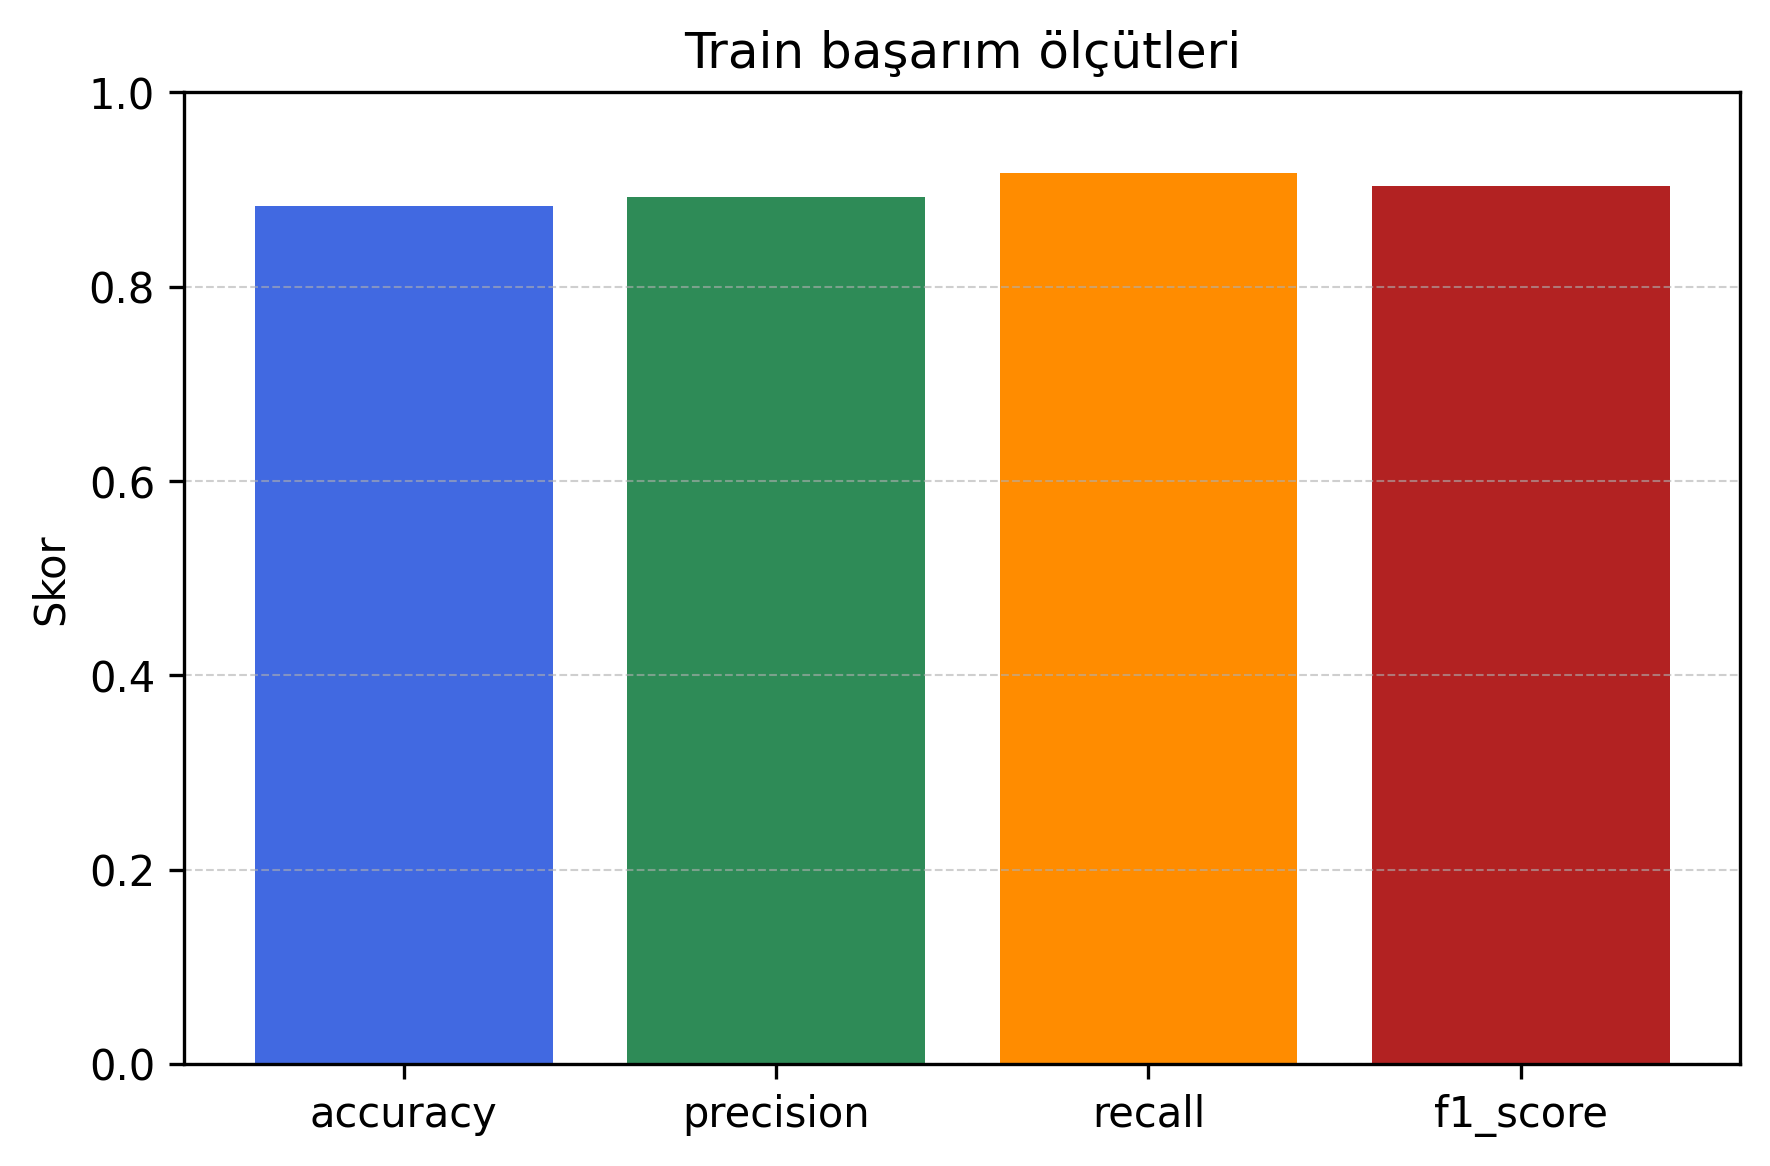
\includegraphics[width=0.9\linewidth]{dataset/gorseller/train_olcutler.png}
  \caption{Eğitim bölümü için accuracy, precision, recall ve F1 skorları.}
  \label{fig:train-bars}
\end{figure}

\begin{figure}[!htb]
  \centering
  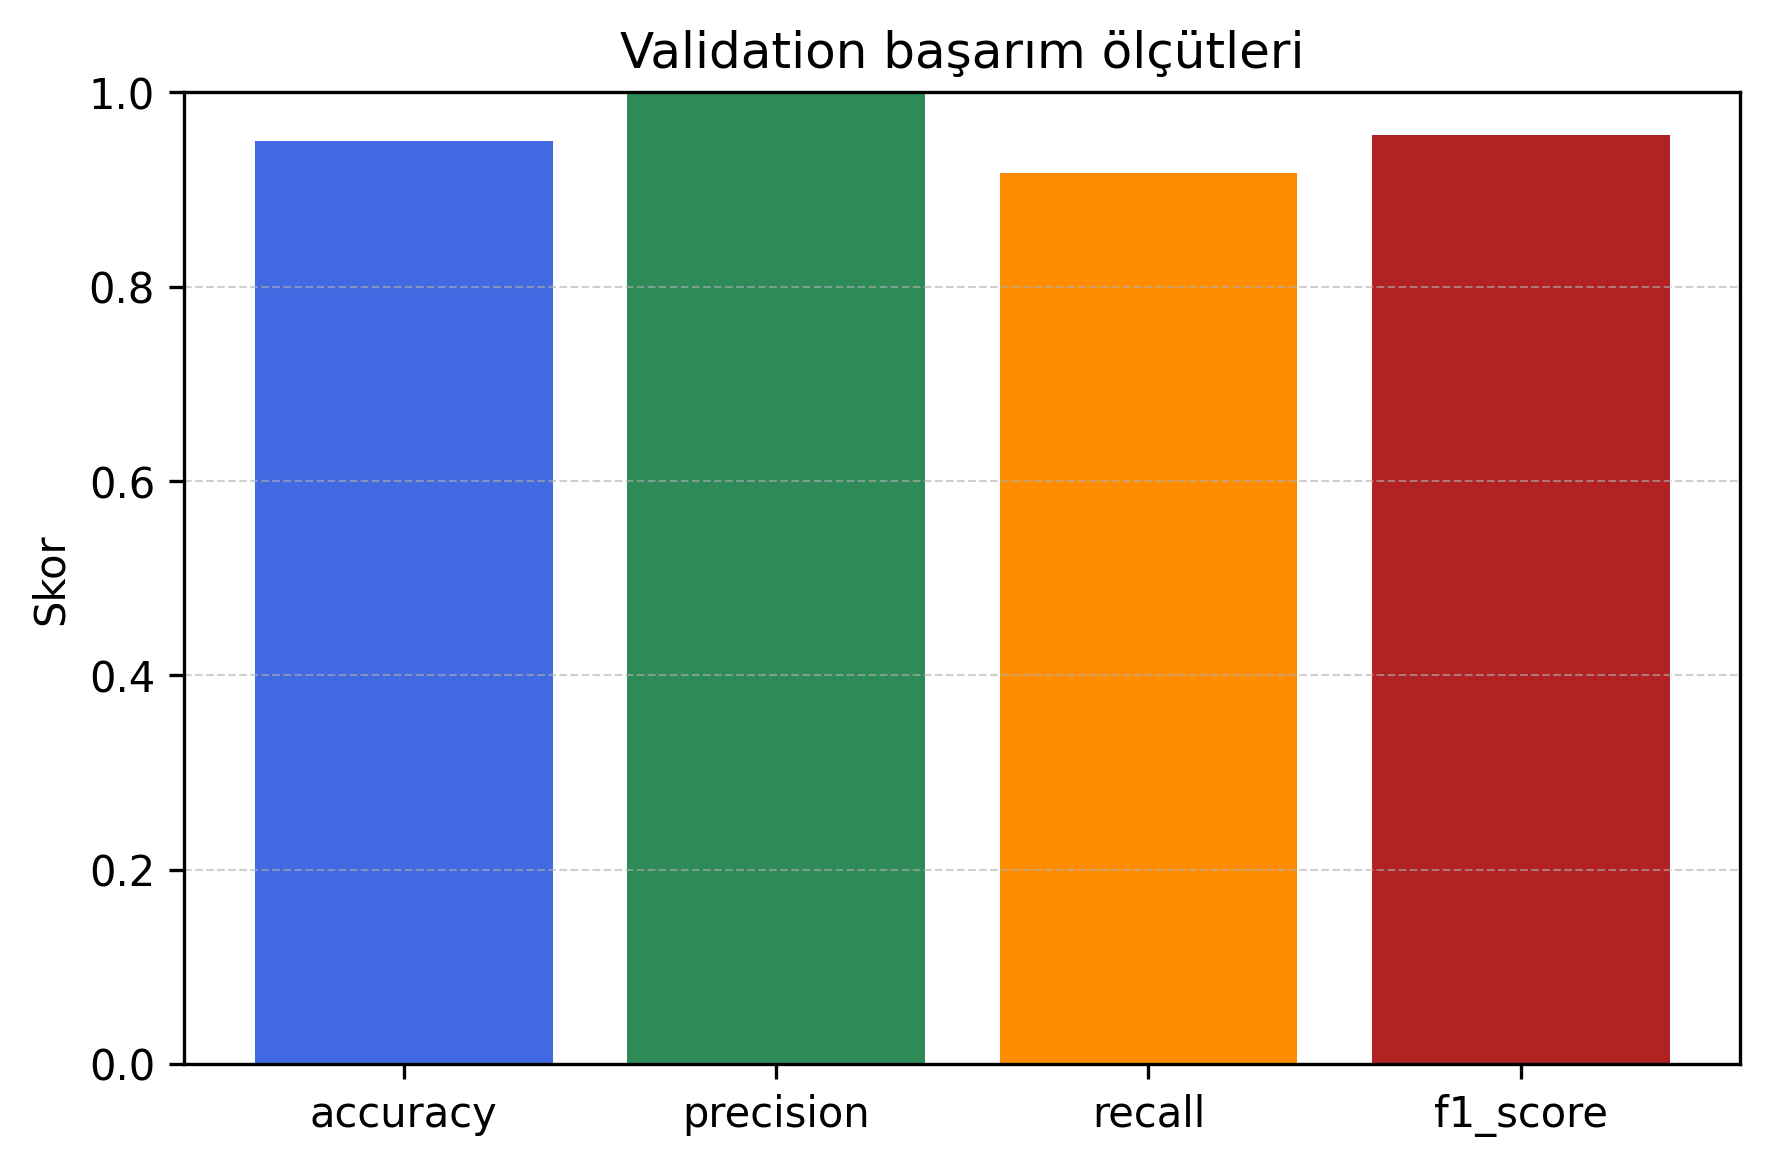
\includegraphics[width=0.9\linewidth]{dataset/gorseller/validation_olcutler.png}
  \caption{Doğrulama bölümü için accuracy, precision, recall ve F1 skorları.}
  \label{fig:val-bars}
\end{figure}

\begin{figure}[!htb]
  \centering
  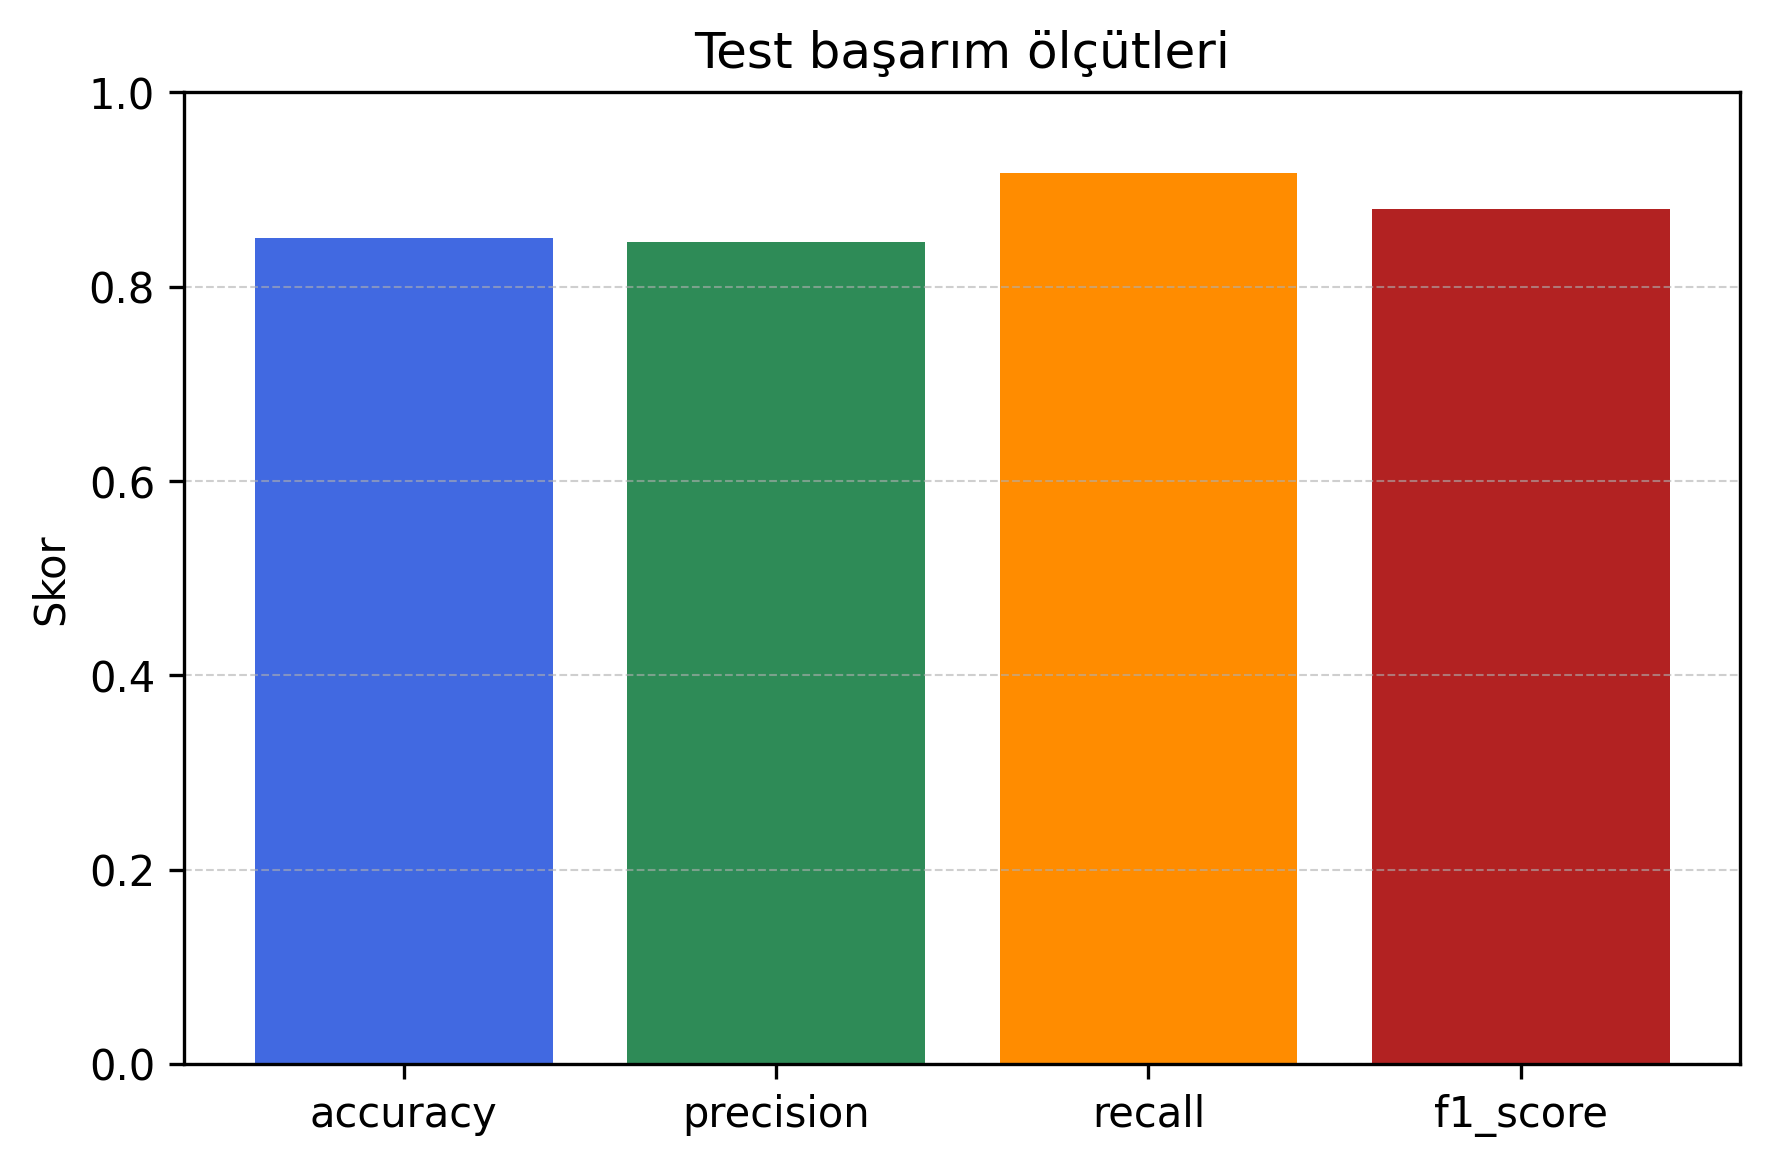
\includegraphics[width=0.9\linewidth]{dataset/gorseller/test_olcutler.png}
  \caption{Test bölümü için accuracy, precision, recall ve F1 skorları.}
  \label{fig:test-bars}
\end{figure}



\section{Sonuç}
Bu çalışmada lojistik regresyon modeli kullanılarak iki sınav puanından işe alım kararı başarılı bir şekilde tahmin edilmiştir. Kayıp ve başarım eğrileri modelin hızlı yakınsadığını ve 500 döngü sonrasında ek eğitim döngülerinin getirisi olmadığını göstermiştir. Bu bulgu, modelin eğitiminde erken durdurma tekniklerinin kullanılabileceğini ve hesaplama kaynaklarının verimli kullanılabileceğini ortaya koymaktadır.

Test kümesi üzerinde elde edilen 0.85 doğruluk, 0.8462 kesinlik, 0.9167 duyarlılık ve 0.88 F1 skoru, modelin görülmemiş veriler üzerinde dengeli ve güvenilir bir başarım sergilediğini ortaya koymaktadır. Özellikle yüksek duyarlılık değeri, modelin işe alınması gereken adayları kaçırma riskinin düşük olduğunu göstermektedir ki bu, işe alım süreçlerinde kritik bir özelliktir.

Eğitim ve doğrulama eğrileri arasında belirgin bir ayrışma gözlenmemesi, doğrulama kaybının erken aşamada kararlı seviyeye inmesi ve doğrulama başarımında çöküş olmaması, modelin \textbf{aşırı uyum (overfitting) göstermediğini} kanıtlamaktadır. Bu durum, lojistik regresyon gibi parametrik modellerin sınırlı kapasitesinin, küçük veri setlerinde regularizasyon görevi görerek doğal bir koruma sağladığını doğrulamaktadır.

Veri setinin tabakalı şekilde bölünmesi ve her bir alt kümenin homojen dağılım sergilemesi, sonuçların güvenilirliğini artırmaktadır. Genel olarak model, basit yapısına rağmen iyi bir genelleme kabiliyeti sergilemektedir ve bu tür ikili sınıflandırma problemleri için pratik bir çözüm sunmaktadır. Gelecek çalışmalarda, özellik mühendisliği (feature engineering) veya polinom özelliklerin eklenmesi gibi yöntemlerle model performansının daha da artırılabileceği değerlendirilmektedir.

\end{document}
